% \documentclass[onecolumn, aps, floatfix]{revtex4-1}
\documentclass{article}

\usepackage[margin=0.75in]{geometry}
\usepackage{listings}
\usepackage{graphicx}
\usepackage{fancyhdr}
\usepackage{amssymb}
\usepackage{amsmath}
\usepackage{caption}
\usepackage{subcaption}
\usepackage{enumerate}
\usepackage{subcaption}
\usepackage{textcomp}
\usepackage{placeins}
\usepackage{blindtext}

\usepackage{color}

\definecolor{mygreen}{rgb}{0,0.6,0}
\definecolor{mygray}{rgb}{0.5,0.5,0.5}
\definecolor{mymauve}{rgb}{0.58,0,0.82}

\lstset{ %
  backgroundcolor=\color{white},   % choose the background color; you must add \usepackage{color} or \usepackage{xcolor}; should come as last argument
  basicstyle=\footnotesize,        % the size of the fonts that are used for the code
  breakatwhitespace=false,         % sets if automatic breaks should only happen at whitespace
  breaklines=true,                 % sets automatic line breaking
  captionpos=b,                    % sets the caption-position to bottom
  commentstyle=\color{mygreen},    % comment style
  deletekeywords={...},            % if you want to delete keywords from the given language
  escapeinside={\%*}{*)},          % if you want to add LaTeX within your code
  extendedchars=true,              % lets you use non-ASCII characters; for 8-bits encodings only, does not work with UTF-8
  frame=single,                    % adds a frame around the code
  keepspaces=true,                 % keeps spaces in text, useful for keeping indentation of code (possibly needs columns=flexible)
  keywordstyle=\color{blue},       % keyword style
  language=Octave,                 % the language of the code
  morekeywords={*,...},            % if you want to add more keywords to the set
  numbers=left,                    % where to put the line-numbers; possible values are (none, left, right)
  numbersep=5pt,                   % how far the line-numbers are from the code
  numberstyle=\tiny\color{mygray}, % the style that is used for the line-numbers
  rulecolor=\color{black},         % if not set, the frame-color may be changed on line-breaks within not-black text (e.g. comments (green here))
  showspaces=false,                % show spaces everywhere adding particular underscores; it overrides 'showstringspaces'
  showstringspaces=false,          % underline spaces within strings only
  showtabs=false,                  % show tabs within strings adding particular underscores
  stepnumber=2,                    % the step between two line-numbers. If it's 1, each line will be numbered
  stringstyle=\color{mymauve},     % string literal style
  tabsize=2,                       % sets default tabsize to 2 spaces
  % title=\lstname                   % show the filename of files included with \lstinputlisting; also try caption instead of title
}

\begin{document}

\title{Lab 6. Oscillator Design and Antenna Measurements }
\author{Albert Wandui \\
\textit{EE 152: High Frequency Systems Lab.}}
\maketitle

% {\let\newpage\relax\maketitle} % Ensures that there is no page break after maketitle

\section*{Introduction}\label{sec:introduction}
The goal of this lab is to design and fabricate a microwave oscillator. In addition, we measured the transmission of a cantenna system and calculated the gain of the antenna. Microwave oscillators convert dc power to RF and are ubiquitous in microwave systems as sources of power. 

We realized our oscillator using negative resistance active devices. These are devices that present a negative input impedance. While positive resistance devices dissipate power, negative resistance devices supply power. For oscillations to begin, the system must be unstable. In this case, fluctuations in the system will build up and drive the circuit to oscillate at a particular frequency. Consider a one port source with reflection coefficient $\Gamma_s$ connected to a load with reflection coefficient $\Gamma_l$. Using Mason's rule the total signal transmitted from the source to the load is given by $1/\left(1 - \Gamma_l \Gamma_s \right)$. From this, we note that as the product of the two reflection coefficients approaches 1, then the system becomes unstable and more and more power is transmitted to the load. This gives us a condition for oscillations to begin, $\Gamma_l \Gamma_s = 1$. We can translate these conditions into limits that the real and imaginary parts of the impedances must satisfy. Note that the impedance of the source (which is an active network) depends on the bias voltage of the source V. At a frequency $\omega$, oscillations will begin if

\begin{align}
    &R_l(\omega) + R_s(V, \omega) = 0 \\
    &X_l (\omega) + X_s(V, \omega) = 0 
\end{align}

The reactance condition sets the frequency of oscillation and the resistance equations gives the gain conditions of the oscillator. In practice, we do not want to barely satisfy the oscillator conditions, so we set the bias of the source so that maximum oscillator power is transmitted to the load. In this case then, we choose $R_l = |R_s|/3$. For transistor based negative resistance oscillators, we first select a potentially unstable transistor for the oscillator. At the output terminal, a matching network is used to make $|\Gamma_{in}| > 1$ looking into the transistor from the load. Here we incorporate series and shunt feedback to increase $|\Gamma_{in}|$ as much as possible. This ensures that ideally, the transistor will oscillate for all passive loads connected to its output. At the remaining terminal, a load network is used to ensure that oscillations do start up at the required frequency. This consists of adding the necessary reactive elements as well as resistance to generate a resonance at the desired frequency. The design of the oscillator network is described in depth in section [\ref{sec:oscdesign}].

An antenna is a circuit element used to couple radiation in free space to an electrical circuit. In effect, antennas act as impedance transformers, matching the impedance of free space (377 $\Omega$) to the impedance of the transmission line ($Z_0$ usually 50 $\Omega$). During transmission, an antenna sets up a radiation pattern consisting of oscillating electric and magnetic fields around its aperture. The radiation pattern of the antenna determines the direction in which the RF power is transmitted. In an ideal antenna all the power input in is transmitted into free space. An omnidirectional antenna transmits power equally in all directions. Usually, antennas have preferred directions in which the power is transmitted. The measure of this directivity is called the gain of the antenna and is usually given in dBi - dB relative to the gain of an isotropic (omnidirectional) antenna with the same power input. An antenna with very high gain directs most of its power into a narrow beam with a small solid angle. In practice, when calculating the gain, we must also account for power losses in the antenna due to impedance mismatch, cable losses, parasitics, resistive and dielectric losses. The effect of these is to lower the gain of the antenna below that of the ideal scenario. 

Antennas are reciprocal devices and thus can be used both to transmit as well as to receive power. The ability of an antenna to intercept radiation is quantified by the effective area of the antenna. There is a simple relation between the effective area of the antenna and the gain of the antenna. For an antenna transmitting radiation with wavelength $\lambda$ and with gain G, the effective area $A_{eff}$ is given by

\begin{equation}
    A_{eff} = \lambda^2 \cdot \frac{G}{4 \pi}.
    \label{eqn:gain}
\end{equation}

Defining the beam solid angle $\Omega = 4\pi/G$, this equation can be rewritten as $A_{eff} \Omega = \lambda^2$. This equation says that at a given transmission frequency, the area solid angle product is the same for all lossless antennas regardless of their design. Thus antenna which produce small beams on sky when transmitting, have large effective areas when receiving radiation. Using this relation, we can compute the total power received by an antenna $P_{RX}$ given the power $P_{TX}$ transmitted by an antenna with a gain $G_{TX}$ and at a distance r away from the receiver. If the receiver has an effective area $A_{eff}$, gain $G_{RX}$ and is receiving at a wavelength $\lambda$ then the Friis transmission equation gives

\begin{align}
    P_{RX} &= \frac{P_{TX}}{4 \pi r^2} \cdot G_{TX} \cdot A_{eff} \\
           &= \left(\frac{\lambda}{4 \pi r}\right)^2 \cdot G_{TX} \cdot G_{RX} \cdot P_{TX}
\label{eqn:friis}
\end{align}

This equation holds as long as the two antennas are in the far field of each other, in unobstructed free space and with no multiple paths between the antennas. In addition, we assume that the antenna bandwidth is narrow enough that a single wavelength is sufficient to describe the radiation and that the polarizations of the fields of the two antenna are well matched.

In this lab, we used a cantenna which is a simple antenna consisting of a cylindrical can of radius a and with a length equal to several times the wavelength that we want to transmit. The cantenna acts as a wave guide. To couple the cantenna to the transmission line, a  $\lambda_g/4$ long coax lead is inserted at a distance equal to $\lambda_g/4$ from the back wall of the can. Here, $\lambda_g$ is the wavelength of the EM mode in the guide. The back wall of the can acts as a short reflecting radiation propagating backwards back towards the probe in phase with radiation from the probe. This focuses the radiation into the direction of the cantenna. The coax lead acts as a quarter wave dipole attached to the cantenna. The propagating modes in the cantenna can be obtained by solving the Helmholtz equations for the E and H fields in cylindrical coordinates. A solution in terms of Bessel functions shows that multiple propagation modes can be supported by a cantenna. However, ideally we'd want to only have 1 mode propagating in the cantenna and care must be taken to avoid exciting higher order modes which would leak power. We chose to operate using the $TE_{11}$ mode which has a mode wavelength of 56.9 mm at 5.9 GHz. Using equation [\ref{eqn:gain}], we can compute the peak gain of the cantenna which is approximately 

\begin{equation}
G_{peak} \approx \left(\frac{2 \pi a}{\lambda_g}\right)^2
\label{eqn:can}
\end{equation}

\section*{Oscillator Design}\label{sec:oscdesign}

To design our oscillator, first we selected the transistor bias point that would give us the least stability at our frequency of oscillation 5.9 GHz. Since the transistor is used in the common base configuration for the oscillator, we needed to convert from the 2 port to 3 port S parameters to get access to all three ports of our transistor. For this, I wrote a short python script which is attached to the end of this report. We found that a bias of 2.5V and 20 mA at the collector worked well. With a 0.5 nH inductor at the base of the transistor, we were able to achieve a stability factor, k = -0.9573 at 5.9 GHz as shown in figure [\ref{fig:inductor_base}]. 

\begin{figure}[!htbp]
    \centering
    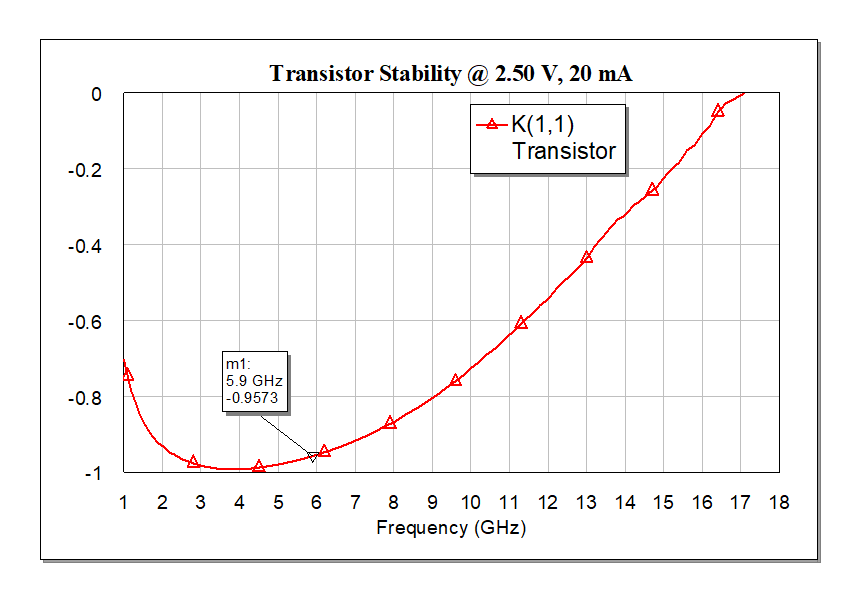
\includegraphics[scale=0.4]{transistor_stable.png}
    \caption{The stability factor of the transistor with a 0.5 nH inductor at the base of the transistor.}
    \label{fig:inductor_base}
\end{figure}

The next step was to design the footprint of the transistor on the board. Working off the datasheet, we spaced the wider emitter pad and the base pad by 45 mil and the collector and second emitter pads by 51 mils. The lengths of the pads were extended slightly to make room for soldering the transistor onto the board. The schematic for the transistor footprint is shown in figure [\ref{fig:footprint}]. As in the lab guide the second emitter pad was terminated using a section of open transmission line on one end and was connected to the larger pad.

\begin{figure}[!htbp]
    \centering
    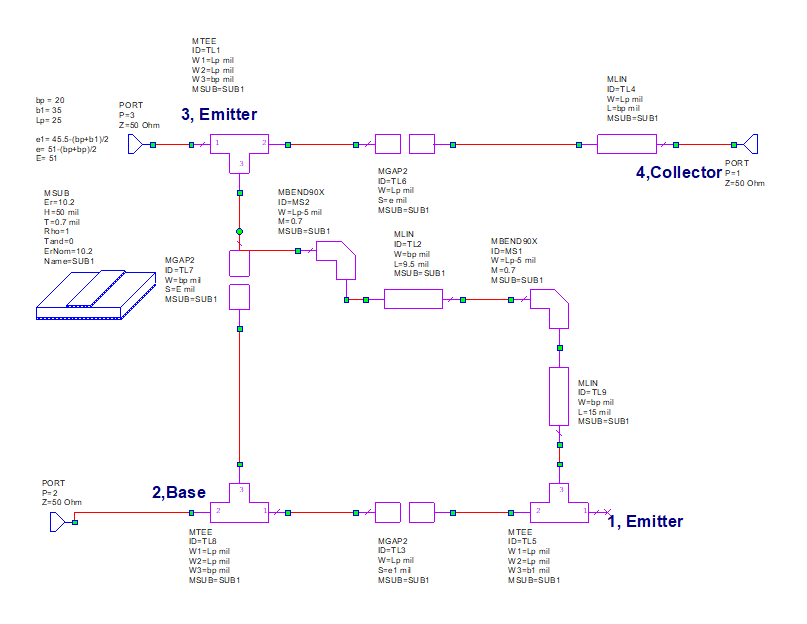
\includegraphics[scale=0.4]{transistor_footprint.png}
    \caption{The footprint of the transistor on the Rodgers Board}
    \label{fig:footprint}
\end{figure}

For the base biasing network, we first made a transmission line equivalent of an inductor. Using a high impedance 25 mil line with characteristic impedance $Z_c\ =\ 68\Omega$, and length $l$ and at a frequency $\omega$, the inductance is given by $\omega L = Z_c \beta l$ where $\beta l$ is the electrical length. Using the TXLine tool to back out the length of the line from the electrical length gives a 10 mil long transmission line. We then added a radial stub of radius 136 mil and 50 \textdegree angle to provide an RF short to ground. At the stub, the transmission line was teed to add the dc base biasing network. To prevent RF power from flowing down the dc bias line, we added a quarter wavelength 187 mil long 10 mil wide (91 $\Omega$) line terminated in a short to ground to act as an open. 10 pF decoupling capacitors were added at the vias and a 14 $k\Omega$ resistor to bias the base of the transistor was added. The full base biasing network is shown in figure [\ref{fig:basebias}].

\begin{figure}[!htbp]
    \centering
    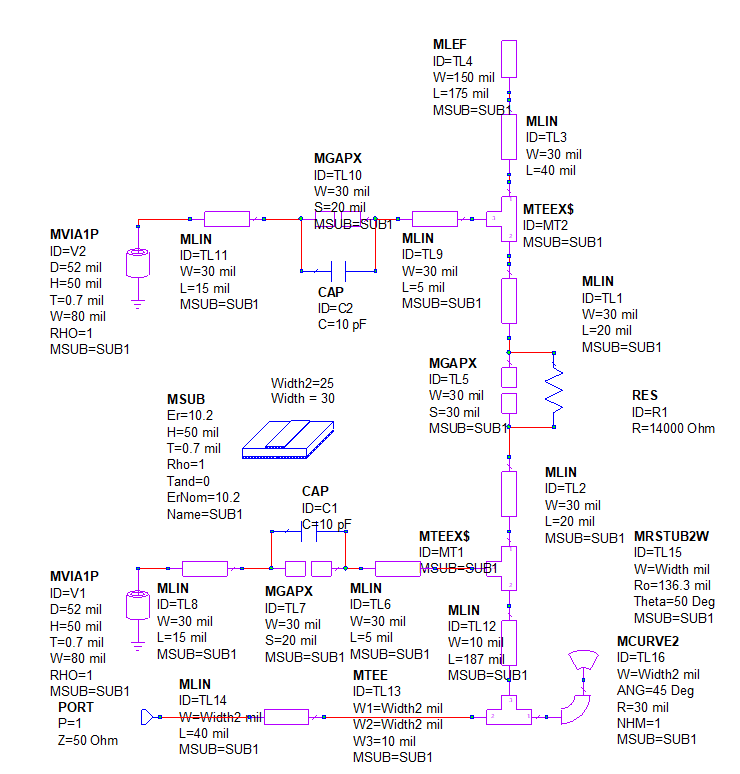
\includegraphics[scale=0.4]{base_biasing_network.png}
    \caption{Schematic of the bias circuit at the base including the RF radial stub and high impedance inductor line.}
    \label{fig:basebias}
\end{figure}

With the base biased so as to make the transistor unstable, we simulated the transistor with the base bias circuit connected at the base. The figure [\ref{fig:collvsemit}] shows a comparison of $S_{11}$ (collector) and $S_{22}$ (emitter) for the transistor network. Indeed, the S parameters are both larger than 1 as expected for an unstable circuit. As shown in the plots, the collector had the higher reflection coefficient and was chosen to be the load. The emitter was the output. To achieve this, the high impedance line of the base inductor was tuned to a 40 mil length.

\begin{figure}[!htbp]
    \centering
    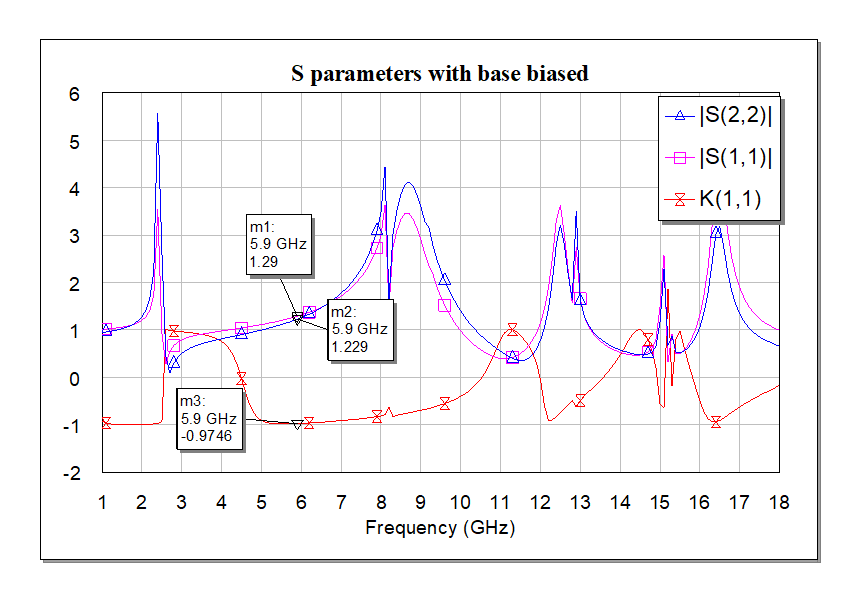
\includegraphics[scale=0.4]{base_biased_S_params.png}
    \caption{Schematic of the bias circuit at the base including the RF radial stub and high impedance inductor line.}
    \label{fig:collvsemit}
\end{figure}

With the emitter selected as the output port, we designed the output network at the emitter to give the correct impedance transformation to ensure that the circuit oscillates for most if not all passive loads and to give a DC bias path to ground. We added a short low impedance line to ensure oscillations for all terminations at the emitter output. To ground the emitter at DC, we added a quarter wavelength 10 mil high impedance line in shunt with the output. The quarter wave length line was terminated with a via to ground to provide an open at RF frequencies. We tuned the length of the line to ensure it presented an open at 5.9 GHz. In addition, we added a 100 pF capacitor at the output to act as a DC Block but providing low impedance at 5.9 GHz. The emitter biasing network is shown in figure [\ref{fig:emitterbias}]. With the output network connected to the emitter port, we plotted the input stability circle seen from the collector. This is shown in figure [\ref{fig:emitterloading}]. From this we can see that we expect oscillations for almost any passive load and certainly for a 50 $\Omega$ load.

\begin{figure}[!htbp]
    \centering
    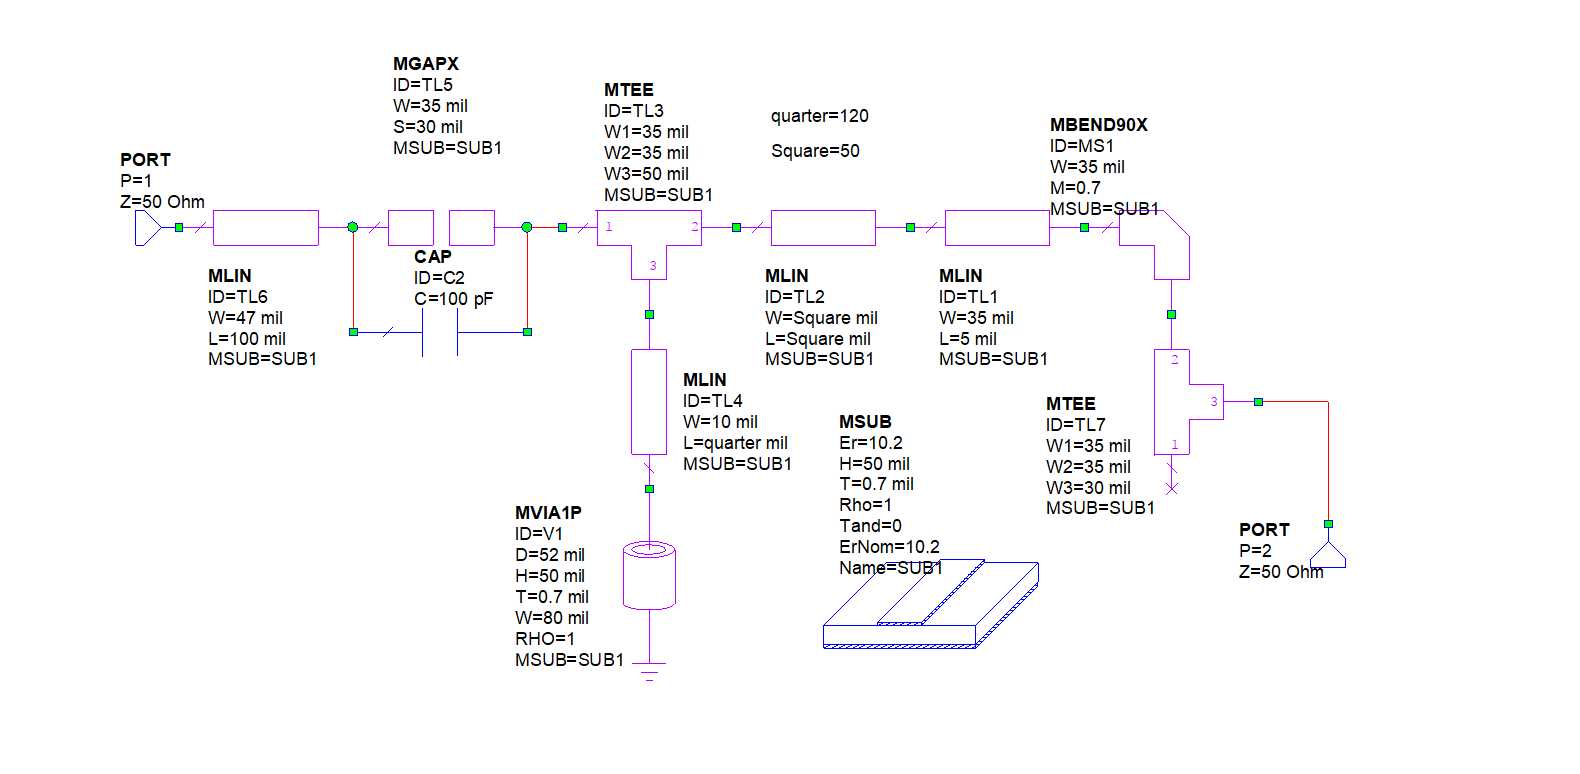
\includegraphics[scale=0.4]{emitter_biasing.png}
    \caption{Schematic of the bias circuit at the emitter.}
    \label{fig:emitterbias}
\end{figure}

\begin{figure}[!htbp]
    \centering
    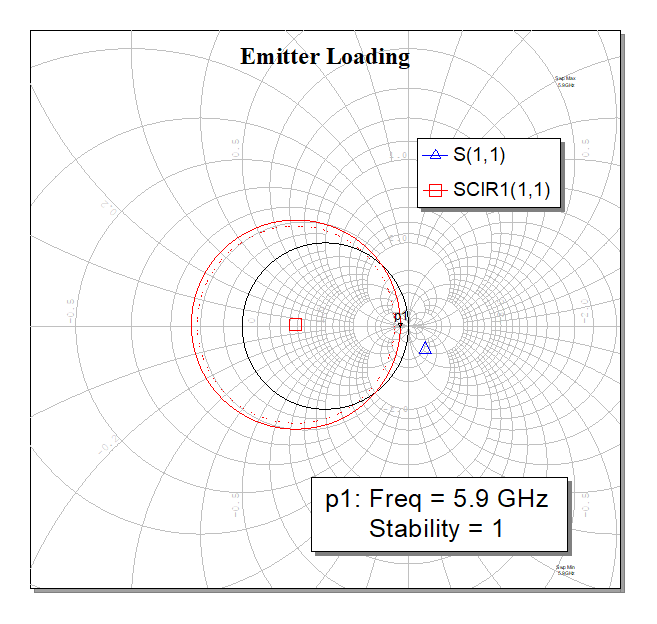
\includegraphics[scale=0.4]{emitter_loading.png}
    \caption{A Smith Chart plot of the stability of the oscillator with the base and emitter biased. The input reflection coefficient seen from the collector is also plotted.}
    \label{fig:emitterloading}
\end{figure}

Lastly, we designed the resonant circuit at the collector. We placed a 50 $\Omega$ load at the output of the emitter and plotted the real and imaginary parts of the input impedance into the collector at 5.9 GHz. This is shown in figure [\ref{fig:inputimpedance}]. The circuit shows a strong negative resistance of -235.6 $\Omega$ and a reactance of -217.9 $\Omega$ at design frequency. We ensure oscillations by conjugately matching the reactance using a 5.9 nH inductor. We also add a 78.5 $\Omega$ resistor which is a third of the absolute value of the real component of the input impedance. With the collector network added, we expect the input impedance looking into the oscillator from the emitter port to resemble that of a resonator. At resonance, the imaginary part of the resonator impedance goes to zero while the real part is maximized. By tuning the inductor value to 3.9 nH and the resistor to 50 $\Omega$, we were able to make the circuit resonant at 5.3 GHz as shown in figures [\ref{fig:collbias1}, \ref{fig:resonator}]
 
 \begin{figure}[!htbp]
    \centering
    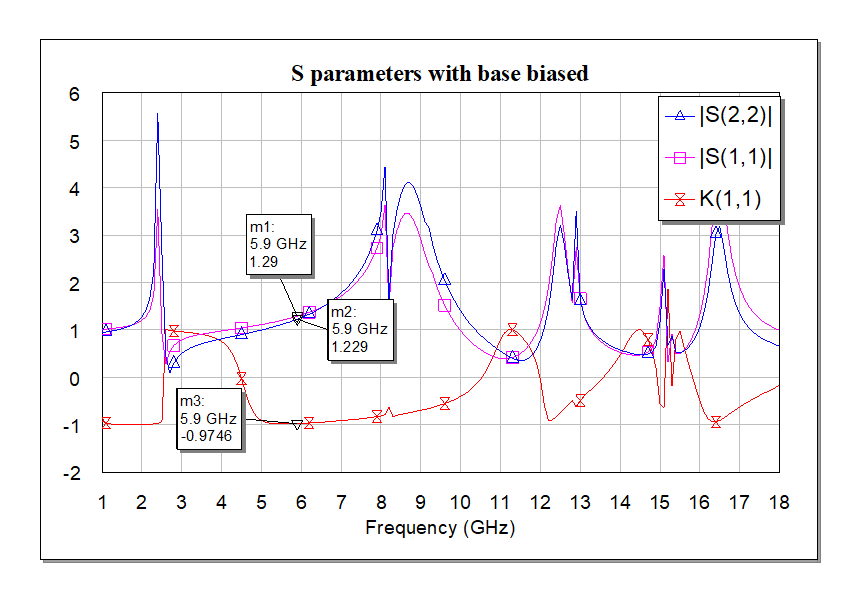
\includegraphics[scale=0.4]{input_impedance.png}
    \caption{The input impedance of the oscillator with a 50 $\Omega$ load at the emitter terminal.}
    \label{fig:inputimpedance}
\end{figure}

\begin{figure}[!htbp]
    \centering
    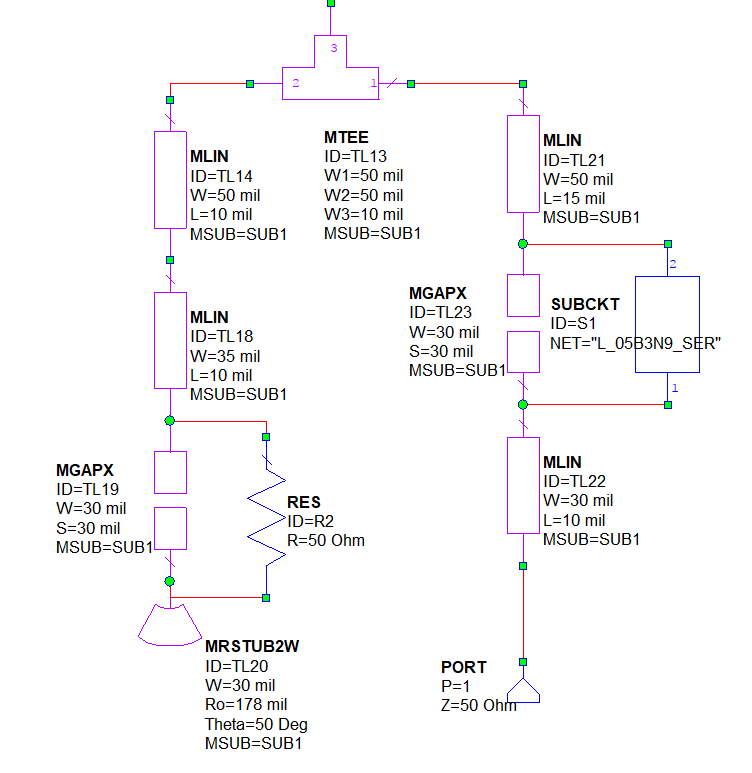
\includegraphics[scale=0.4]{collector_bias_1.png}
    \caption{Resistance and Inductance used to ensure oscillation in the collector.}
    \label{fig:collbias1}
\end{figure}

With the inductors and resistors in place, we added in the bias network for the collector. Again, we used quarter wave high impedance tlines with vias to ground to provide RF opens. At the tees we added radial stubs to provide shorts to ground for the RF signals. Decoupling capacitors were also used at the vias and a 10 $\Omega$ bias resistor. The bias network is shown in figure [\ref{fig:collbias2}]. With all the circuit components completed, we generated the final layout for our oscillator for fabrication. As shown in figure [\ref{fig:resonator}], our circuit could also possibly oscillate at 2.7, 12.2 and 14.1 GHz. While in our design, these oscillations were subdominant, we noted that it was possible that due to additional effects introduced during the circuit assembly, we could instead end up exciting oscillations at frequencies different from the targeted one.
\begin{figure}[!htbp]
    \centering
    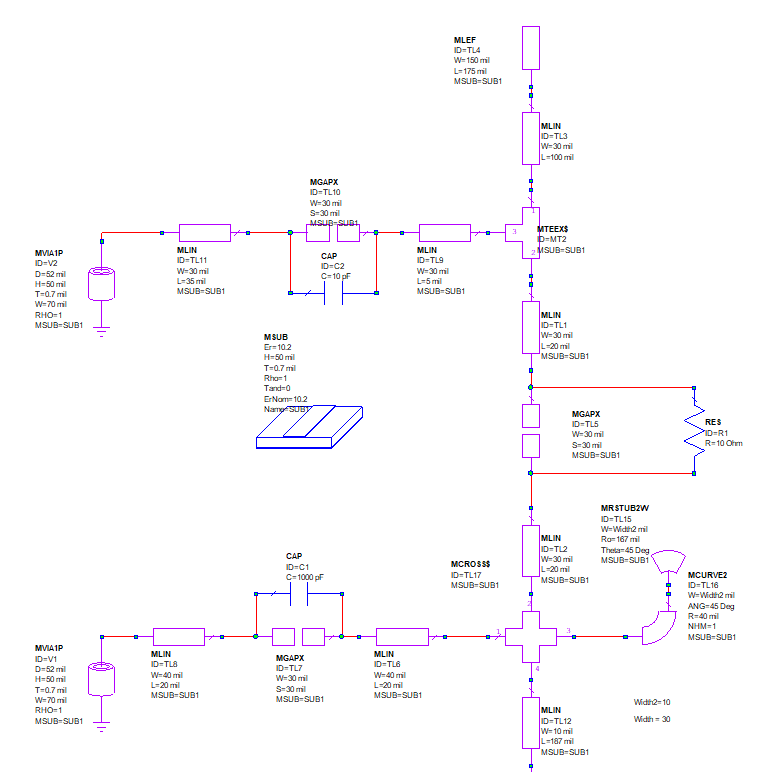
\includegraphics[scale=0.4]{collector_bias_2.png}
    \caption{A schematic of the collector bias network.}
    \label{fig:collbias2}
\end{figure}

\begin{figure}[!htbp]
    \centering
    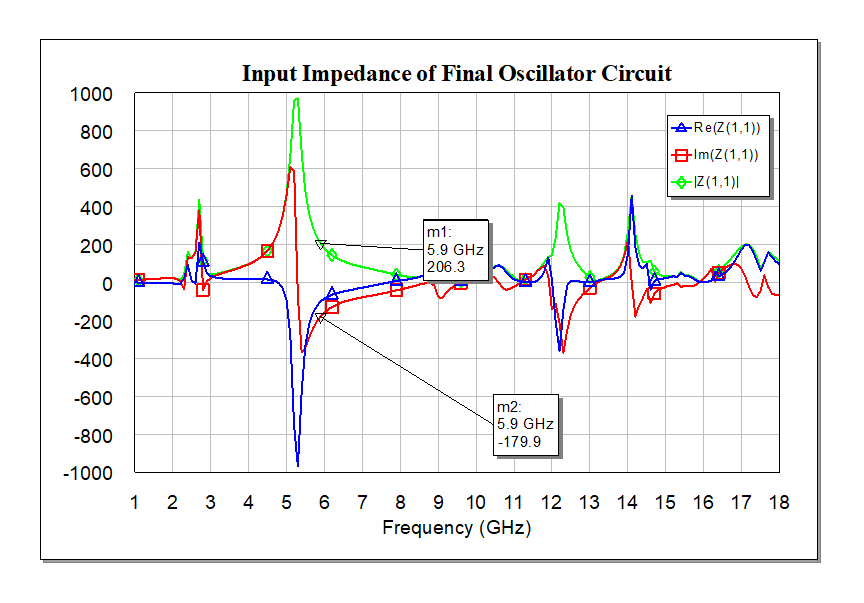
\includegraphics[scale=0.4]{resonator.png}
    \caption{Input impedance of the oscillator as seen from the emitter for the final circuit.}
    \label{fig:resonator}
\end{figure}


\section*{Oscillator Measurements}\label{sec:oscmeas}

To test our oscillator circuit, we first populated the board with all the required 0402 resistors, inductors and capacitors as per the design. The populated circuit board is shown in figure [\ref{fig:oscsetup}]. The FFox was configured to SA mode with a frequency range of 0 to 18 GHz. The two DC supplies for the oscillator were set to 3.5 V OVP and 0.1A OCP. We then hooked up the output of the oscillator to port 2 of the FFox and used the BNC cables with suitable adapters to connect the base and collector ports to the power supplies as shown in figure [\ref{fig:oscmeas}]. We slowly ramped up the voltage output of the power supply until we reached 20 mA collector current. For our initial measurements with a 3.9 nH inductor at the collector, we measured oscillations at 11.7 GHz about 6 GHz too high. We increased the collector inductance to 7.5 nH to achieve a final oscillation frequency of about 6.4 GHz. Due to time constraints, we were not able to make smaller adjustments to the inductance to perfectly match the 5.9 GHz target.

\begin{figure}[!htbp]
    \centering
    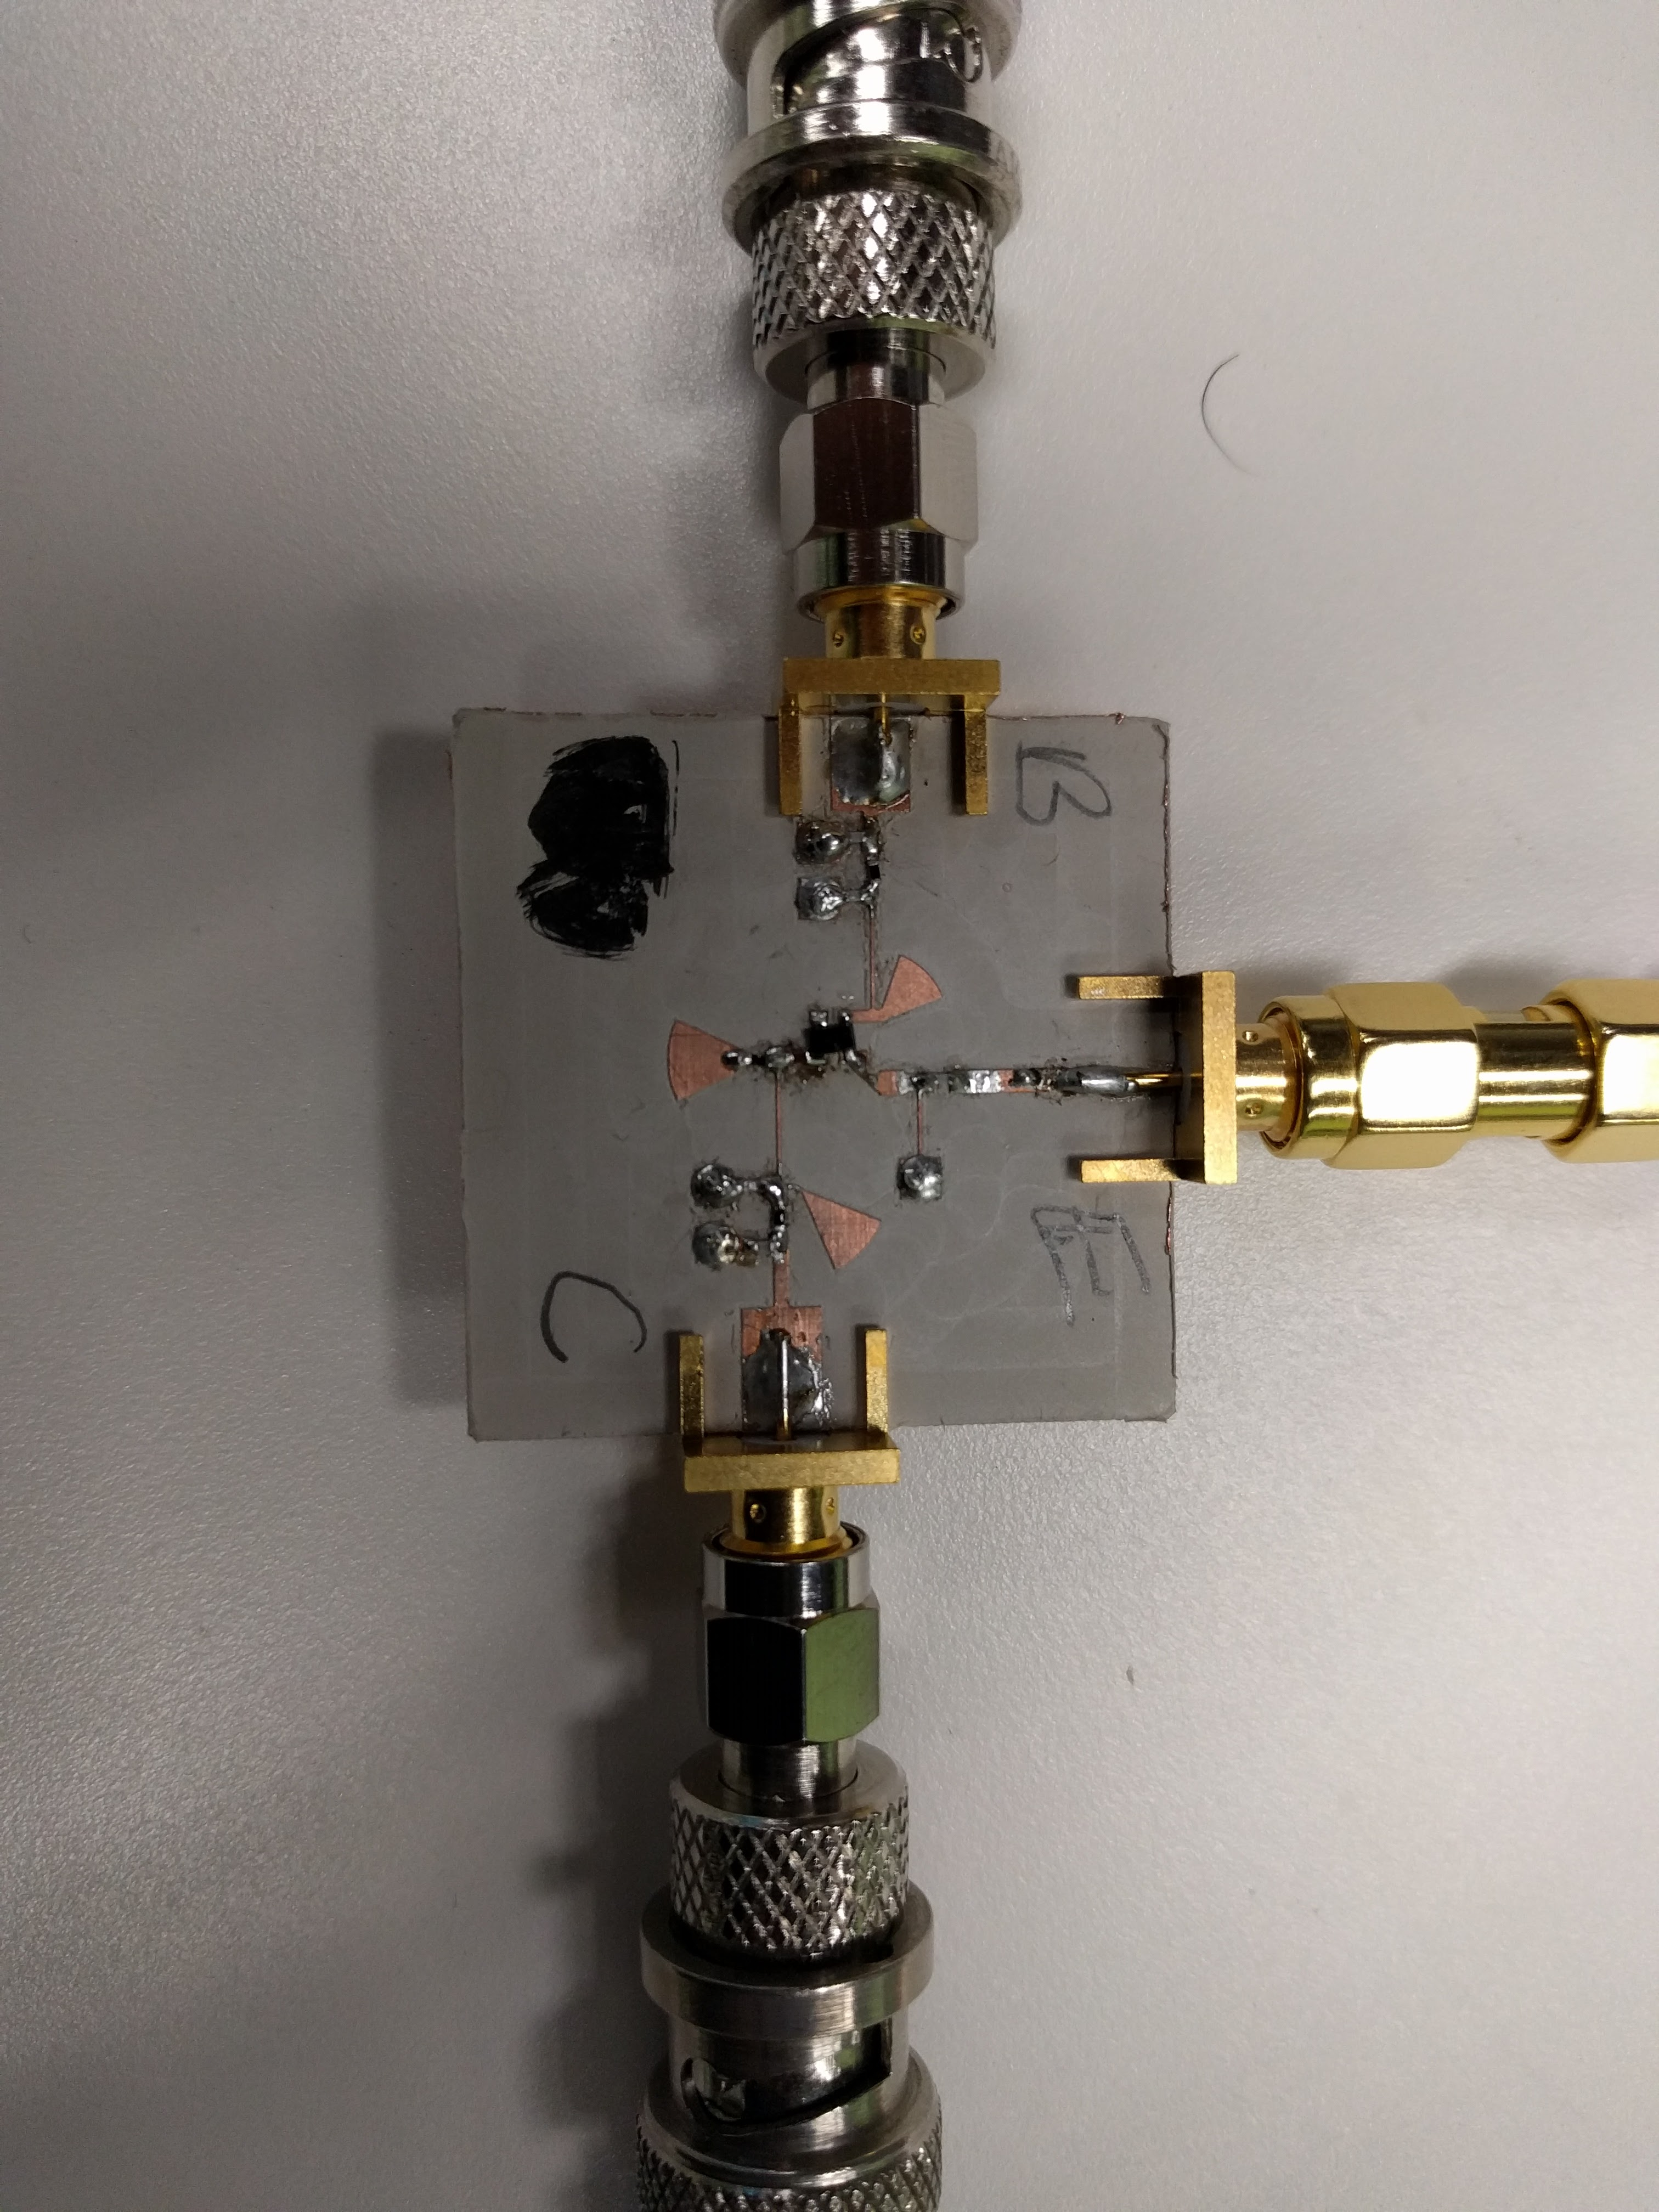
\includegraphics[scale=0.04]{oscillator.jpg}
    \caption{The oscillator circuit board populated with all the components.}
    \label{fig:oscsetup}
\end{figure}

\begin{figure}[!htbp]
    \centering
    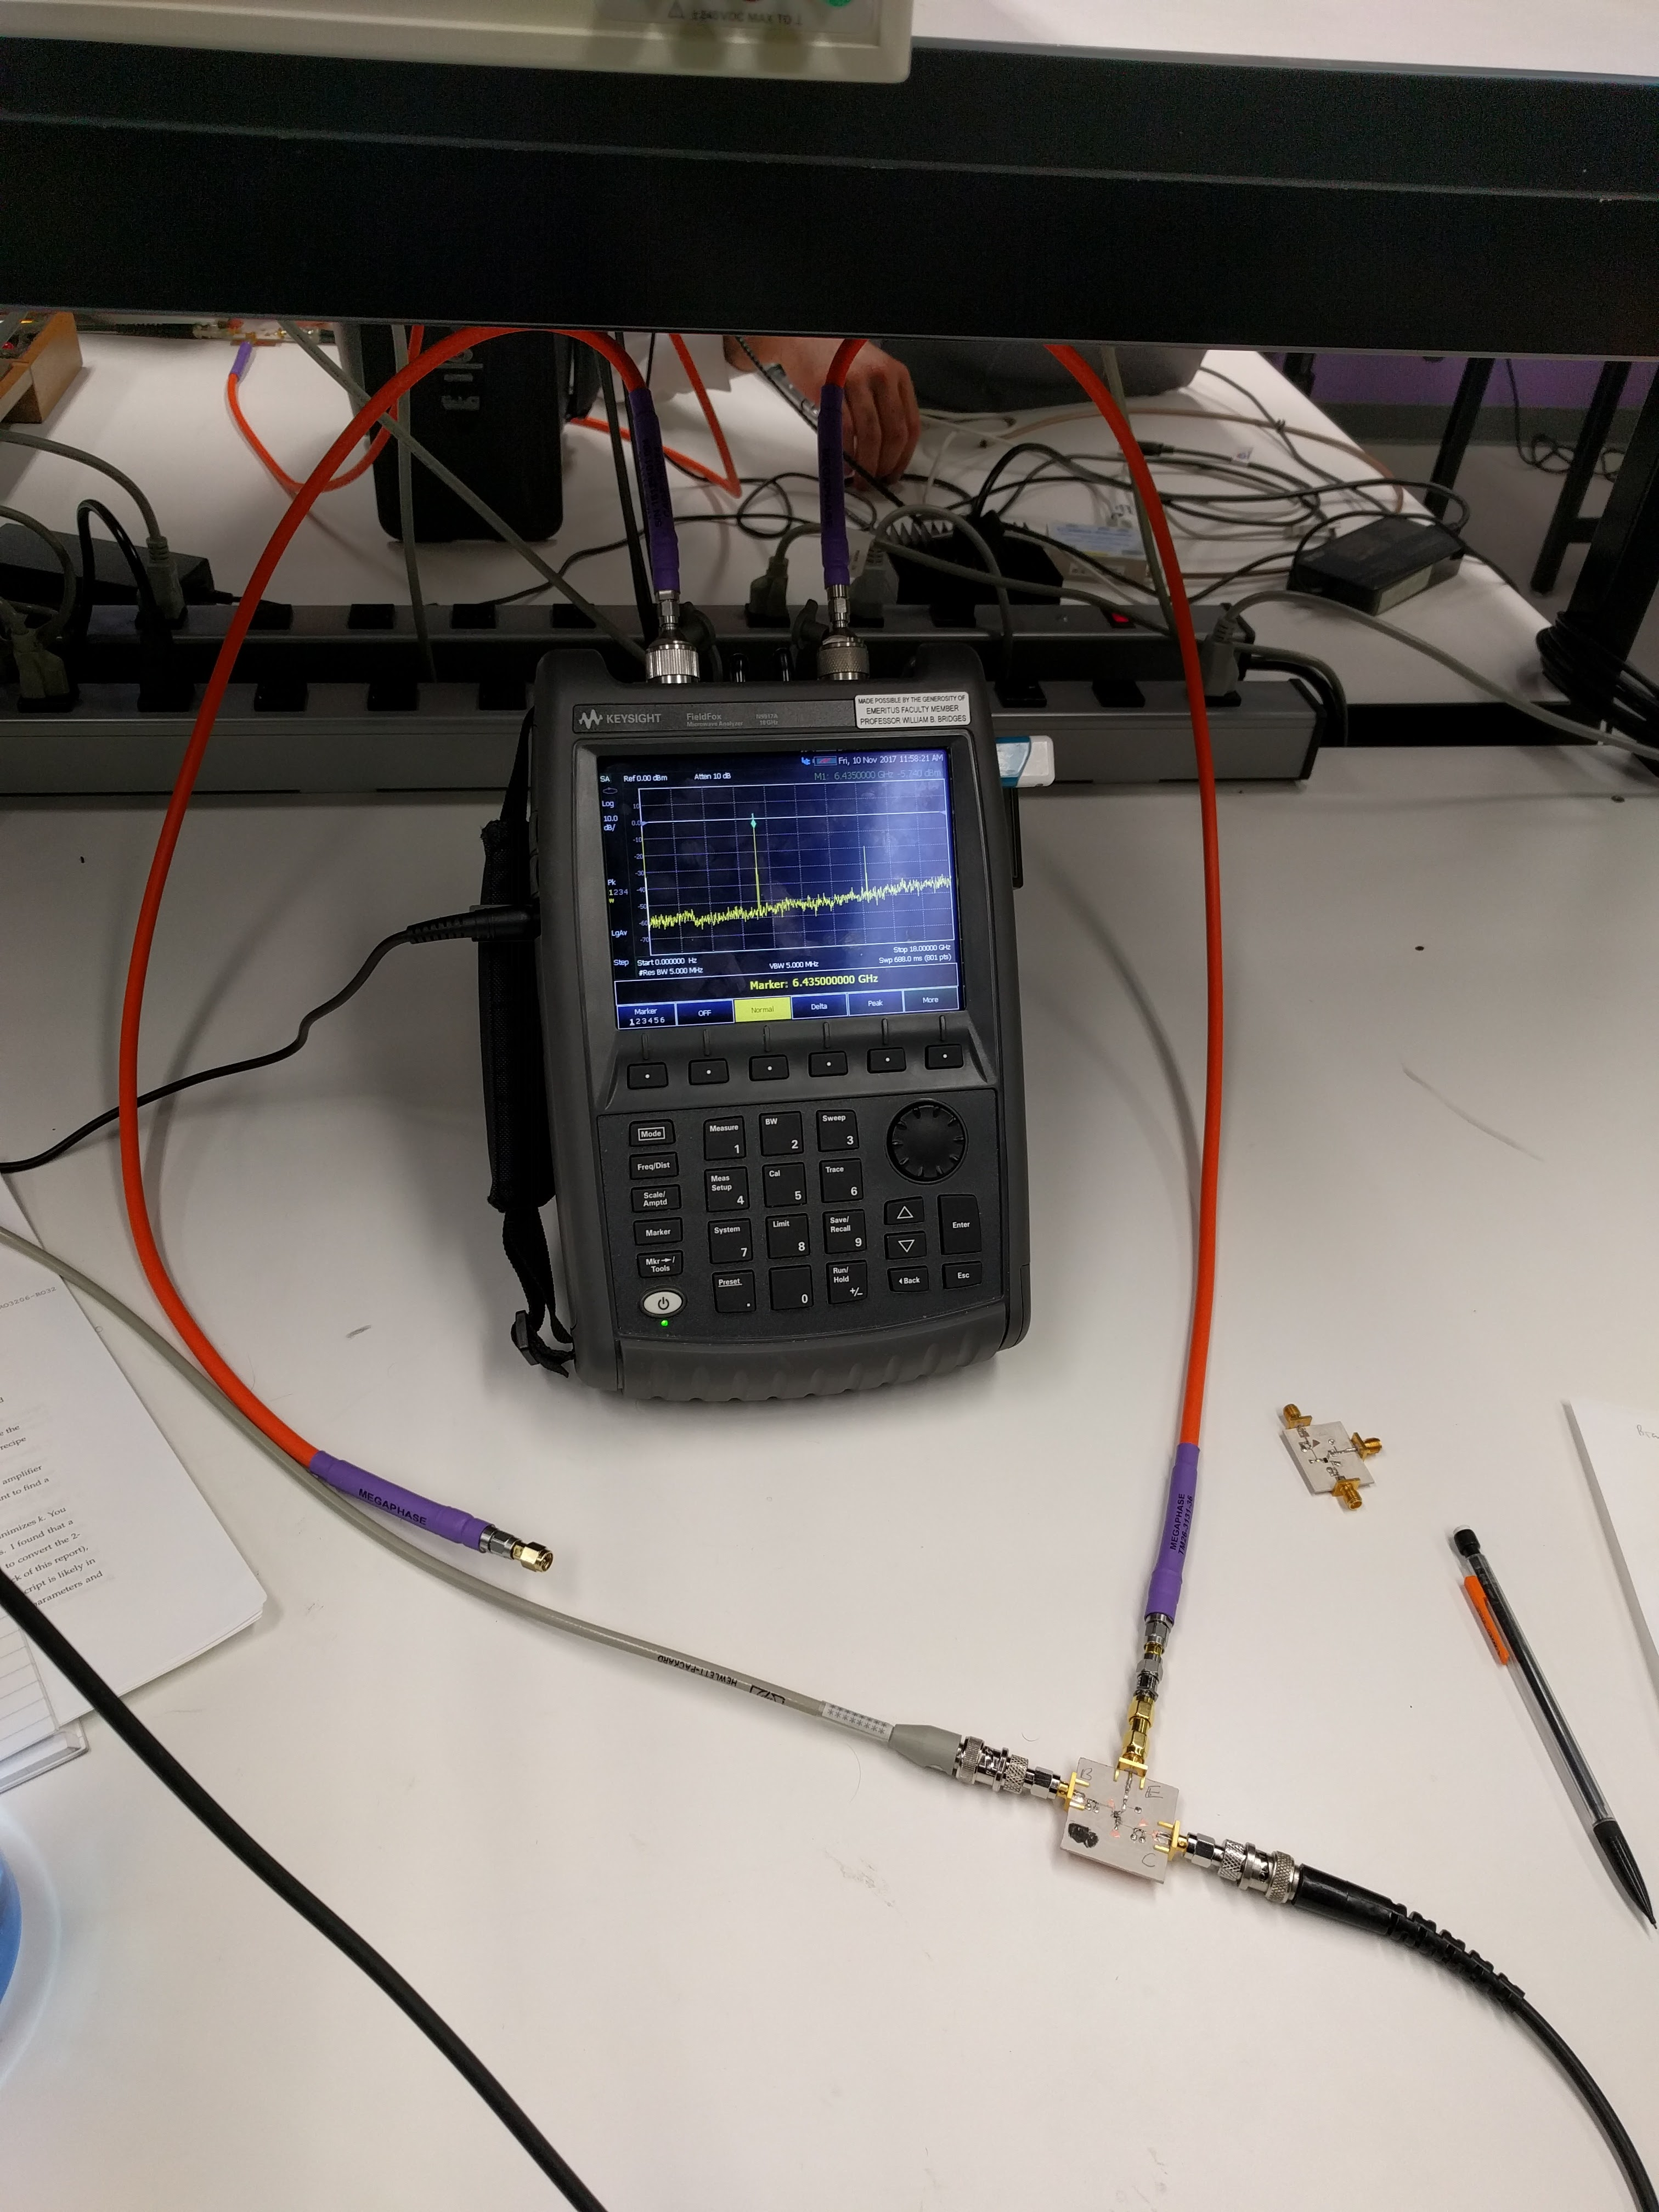
\includegraphics[scale=0.04]{osc_meas_setup.jpg}
    \caption{Measuring the spectral response of the oscillator using the FFox.}
    \label{fig:oscmeas}
\end{figure}

\section*{Antenna Measurements}\label{sec:cantmeas}

We used two cantennas; one setup for transmit and the other setup for receive for this measurement. We assumed that both cantennas have identical gain. The two cantenna setups were positioned 1 m apart as measured in lab. We setup the Hittite signal generator as the power source providing 10 dBm output to the antenna at 5.9 GHz. We expected about a 1 dB loss due to the cables between the antenna and the signal generator. On the receive side, we set the frequency of the power sensor to 5.9 GHz and adjusted the receiver so that the polarizations of the two antenna were well aligned. We adjusted the angle and the horizontal and vertical positions of the receiver until the signal measured on the power sensor was maximized. The measurement setup is shown in figure [\ref{fig:cantennasetup}].

\begin{figure}[!htbp]
    \centering
    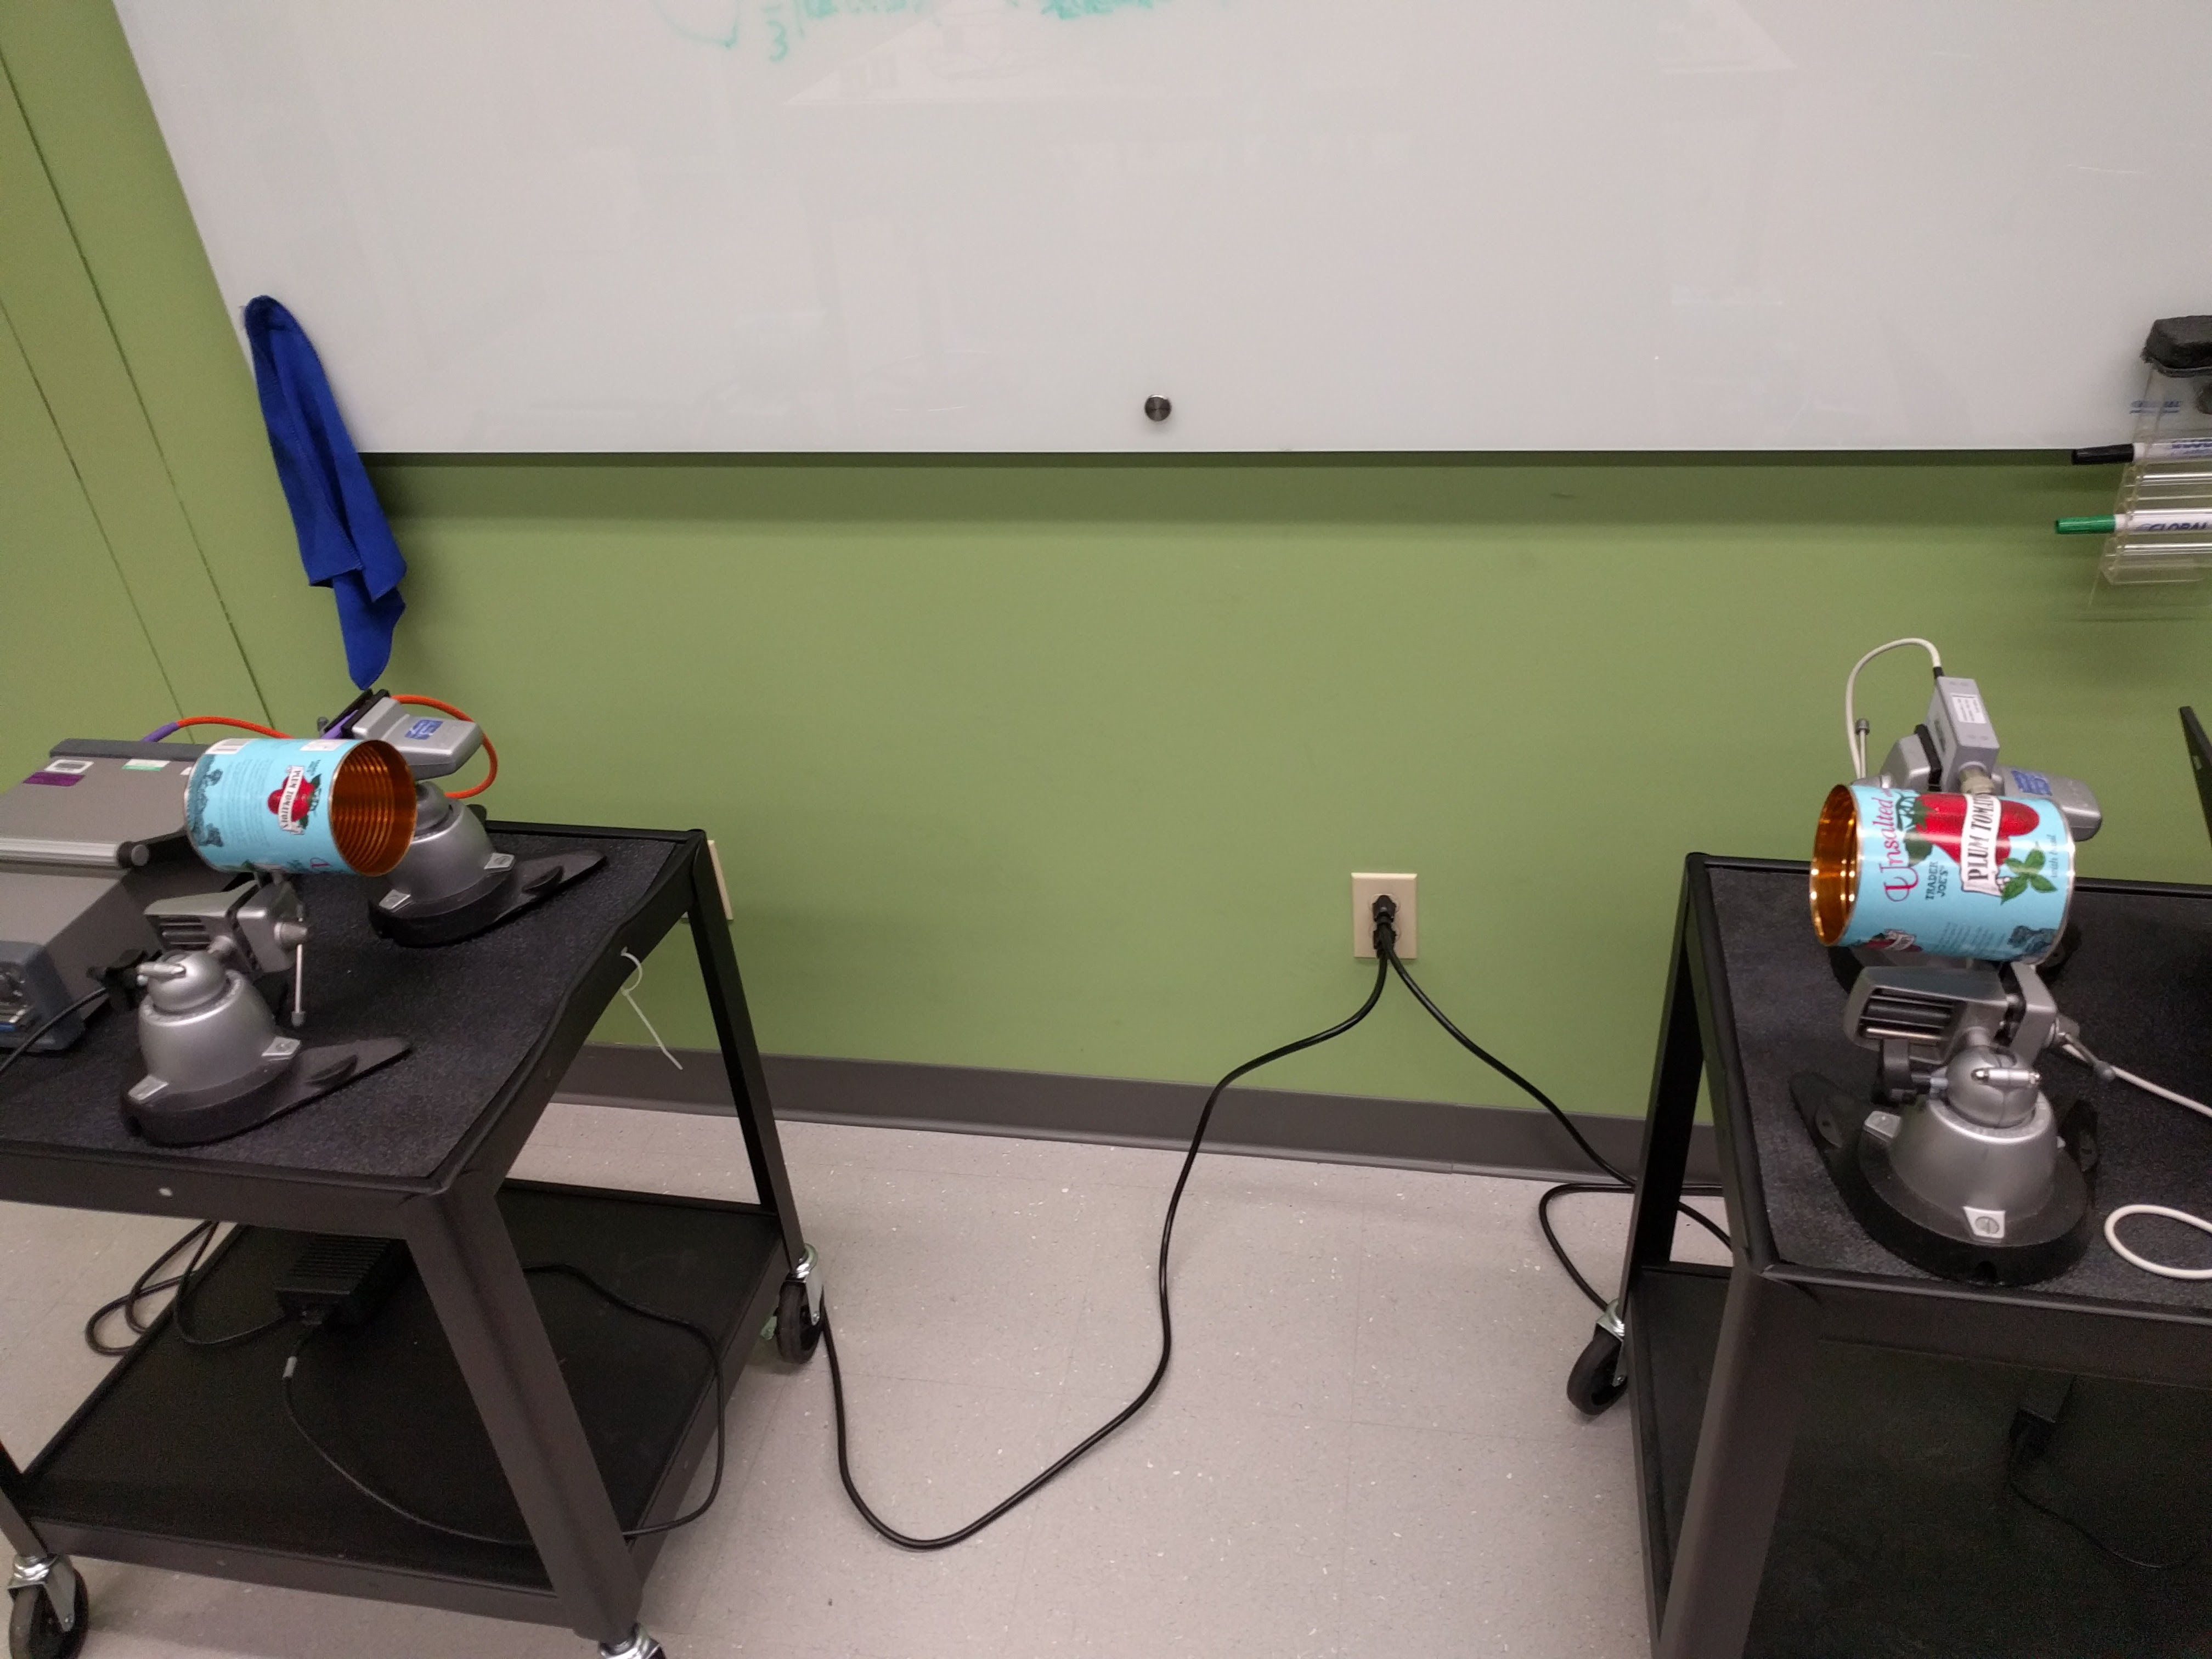
\includegraphics[scale=0.04]{cantenna.jpg}
    \caption{Transmitter and receiver setup for measuring the gain of the cantennas.}
    \label{fig:cantennasetup}
\end{figure}

\section*{Analysis}\label{sec:analysis}

The table [\ref{tab:oscillator}] summarizes the parameters of the oscillator during each tuning step. From the table, we see that the output power increased as we approached the desired oscillation frequency. In figure [\ref{fig:11GHz}], the spectrum of the oscillator with no tuning is shown. As expected, by increasing the inductance by a factor of about 2 we were able to decrease the resonant frequency significantly to more closely approach the design target. The final spectrum with the fundamental peak at 6.44 GHz is shown in figure [\ref{fig:6GHz}]. In this plot, the second harmonic is also clearly visible. The fundamental peaks at -5.64  dBm while the second harmonic peaks at -19.59 dBm. Thus the second harmonic at 12.88 GHz is at -13.95 dBc. The third harmonic was just outside of the measurement range. 

\begin{table}[!htbp]
\begin{tabular}{| c | c | c | c |}
\hline
Frequency [GHz] & Power [dBm] & Resistor [$\Omega$] & Inductor [nH] \\
\hline
\hline
11.77 & -9.61 & 50 & 3.9 \\
\hline
6.44 & -5.64 & 50 & 7.5 \\
\hline
\end{tabular}
\caption{A summary of the oscillator parameters at each tuning step.}
\label{tab:oscillator}
\end{table}

While the resonant frequency was initially much higher than the design specification, we noted that by pressing down on the radial stub at the base, we could excite multiple oscillations over a wide frequency range from about 3 GHz all the way to 11 GHz. Our suspicion is that the close proximity between the radial stub at the base and the bias lines to the transistor base port created some coupling that was not well captured in the design. In addition, as we noted in the design section, many resonant peaks were evident in the final plots of our circuit design. It is likely then that within the tolerances of the circuit assembly and soldering, we shifted the relative strengths between the resonant peaks making the high frequency peak at 11.8 GHz the dominant oscillation mode in the circuit. However, with more time, we could have further adjusted the inductance at the collector to meet design target.

\begin{figure}[!htbp]
    \centering
    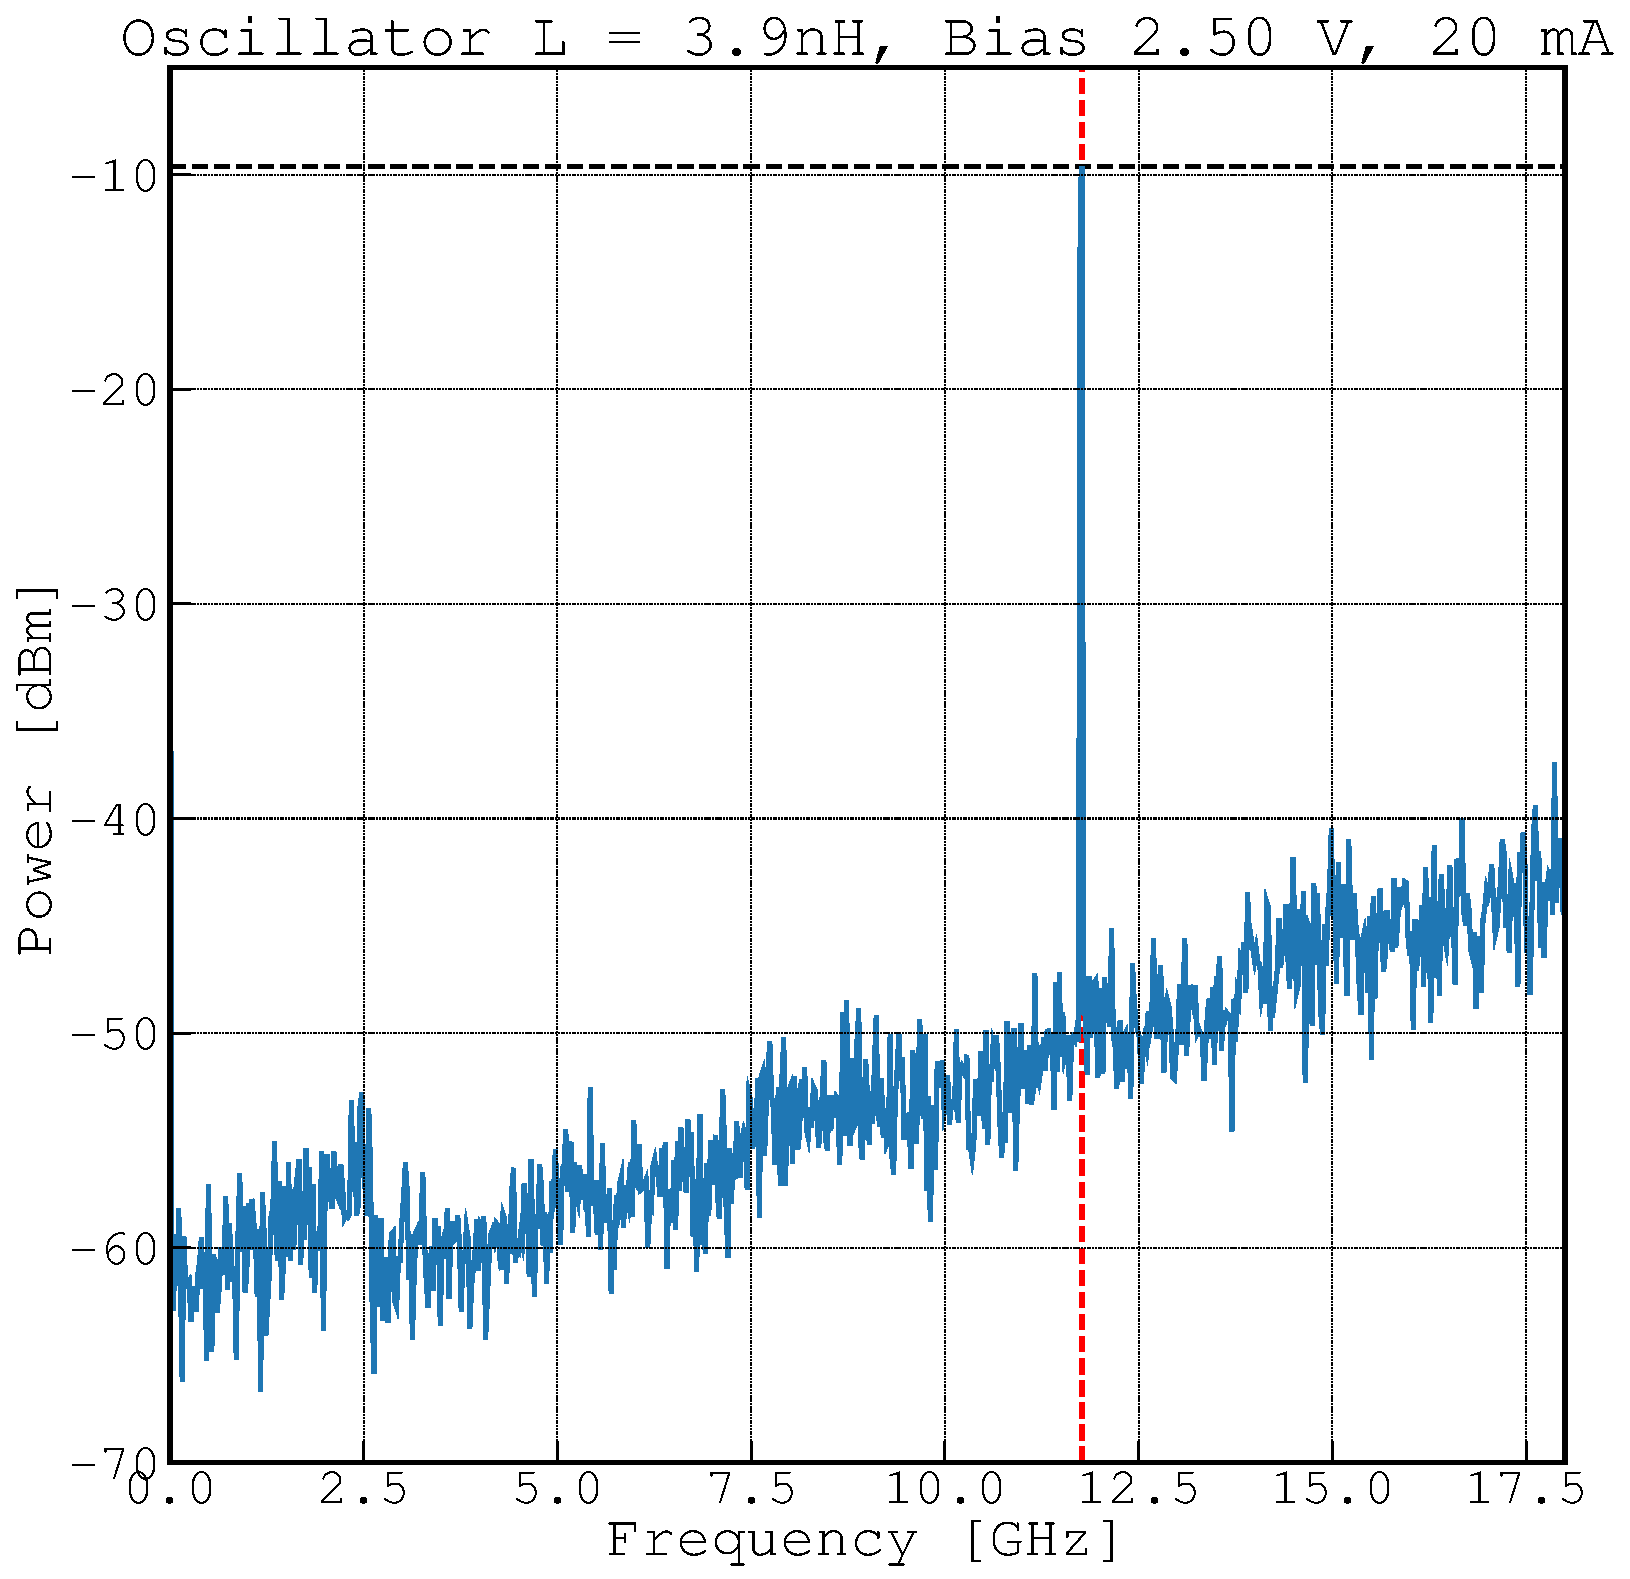
\includegraphics[scale=0.35]{11GHz_plot.pdf}
    \caption{Initial spectral response of the oscillator with a strong oscillation at 11.77 GHz.}
    \label{fig:11GHz}
\end{figure}

\begin{figure}[!htbp]
    \centering
    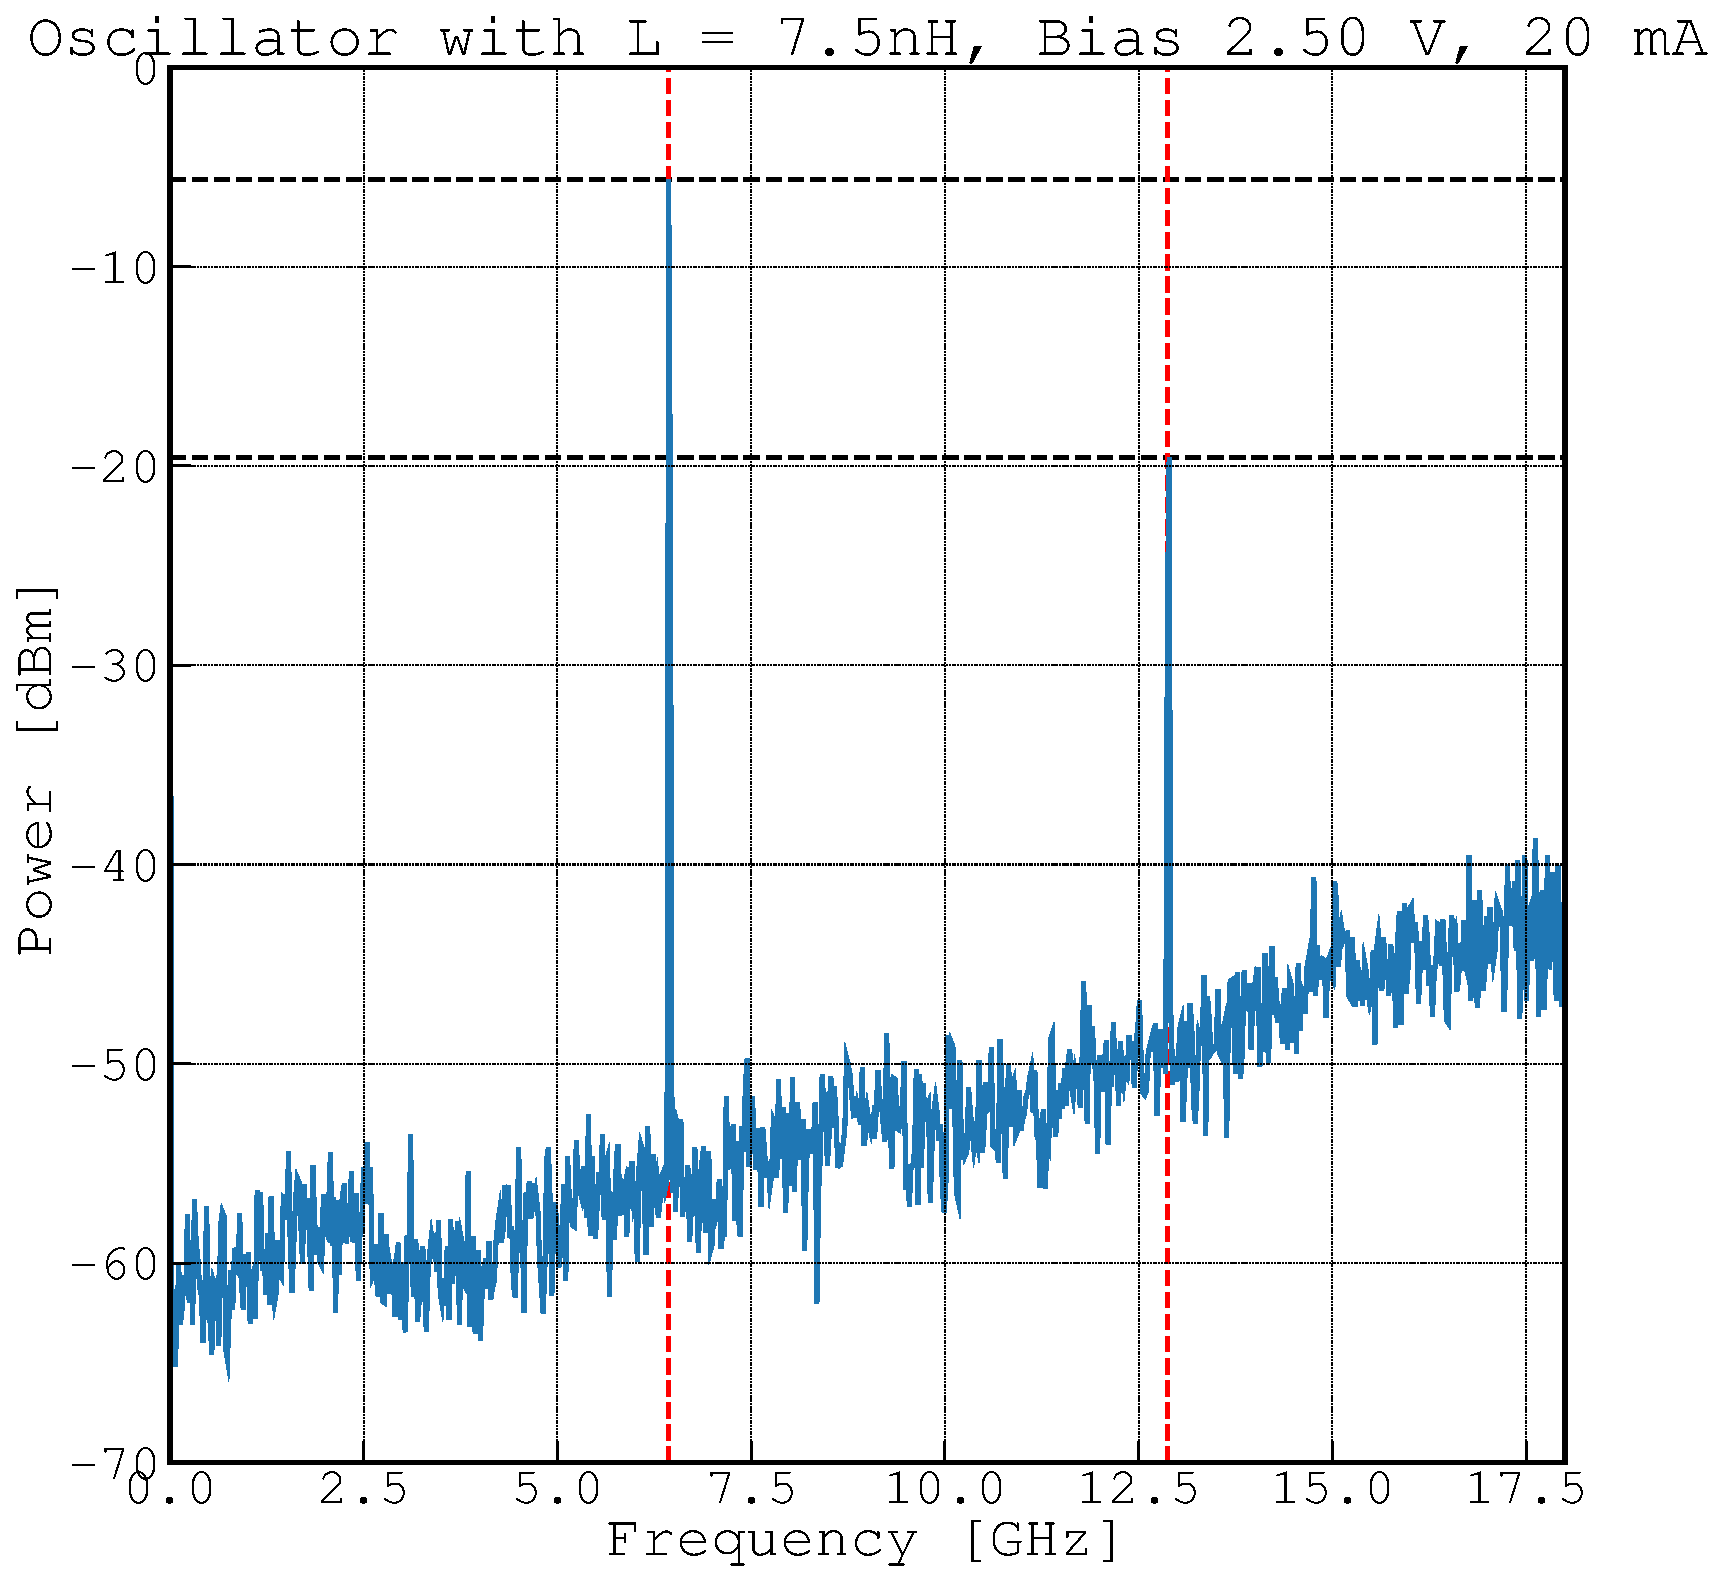
\includegraphics[scale=0.35]{6GHz_plot.pdf}
    \caption{Spectral response of the oscillator after tuning to achieve oscillation at 6.44 GHz.}
    \label{fig:6GHz}
\end{figure}

For the antenna measurements, the maximum power at the receiver was measured to be at -28.4 dBm with a 1m spacing between the two antennas. Using the Friis formula in equation [\ref{eqn:friis}], we can back out the gain of the two antenna. Expressing the power in dBm, and with the assumption that the two gains are equal; $G_{RX} = G_{TX} = G$, we obtain the following equation for the gain

\begin{equation}
    2 G = P_{RX} - P_{TX} - 20 \log_{10} \left[\frac{\lambda}{4 \pi r}\right]
\end{equation}

Now, $P_{TX}$ = 10 dBm - 1 dBm attenuation = 9 dBm. r = 1m, and $\lambda$ is the free space wavelength of radiation at 5.9 GHz which is 50.85 mm. Thus 2 G = -28.4 dBm - 9 dBm - (-47.86 dB). Solving for the gain gives G = 5.23 dBi. For a 4" diameter can, the peak gain expected from equation [\ref{eqn:can}] is about 14.98 dBi. Thus we measured much lower gain than expected. This could be explained if we were indeed off the peak of the transmitted beam. The cart on which the antenna were setup limited the range over which we could scan the antenna since the wheels would slide and set in particular positions. In addition, the peak gain of a cantenna would in practice be much lower than the approximated value due to the excitation of different waveguide modes that rob power from the mode for which the antenna was designed. Numerical modelling of the cantenna would be needed to more accurately account for these effects and better estimate the peak gain of the cantenna. Even so, we noted that our cantenna has a much higher gain than even a dipole antenna (1.76 dBi) and could be built at a fraction of the cost of more comprehensive higher gain horn antennas.  

\section*{File Conversion Code}

I've attached my python code for converting s2p to s3p files. Note that I reformatted the code to fit it better into the page.
\lstinputlisting[language=Python]{fileconverter.py}

\section*{Conclusions}
In this lab, we successfully built and characterized an oscillator operating at RF frequencies. This was an important step towards the final project where we will be implementing a voltage controlled oscillator for our doppler radar system. In addition, we learned how to measure the gain of the cantenna, a procedure that we will repeat with our own cantenna designs for our final project.
\end{document}